\documentclass{standalone}
\usepackage{tikz}
\usetikzlibrary{patterns, positioning}

\begin{document}
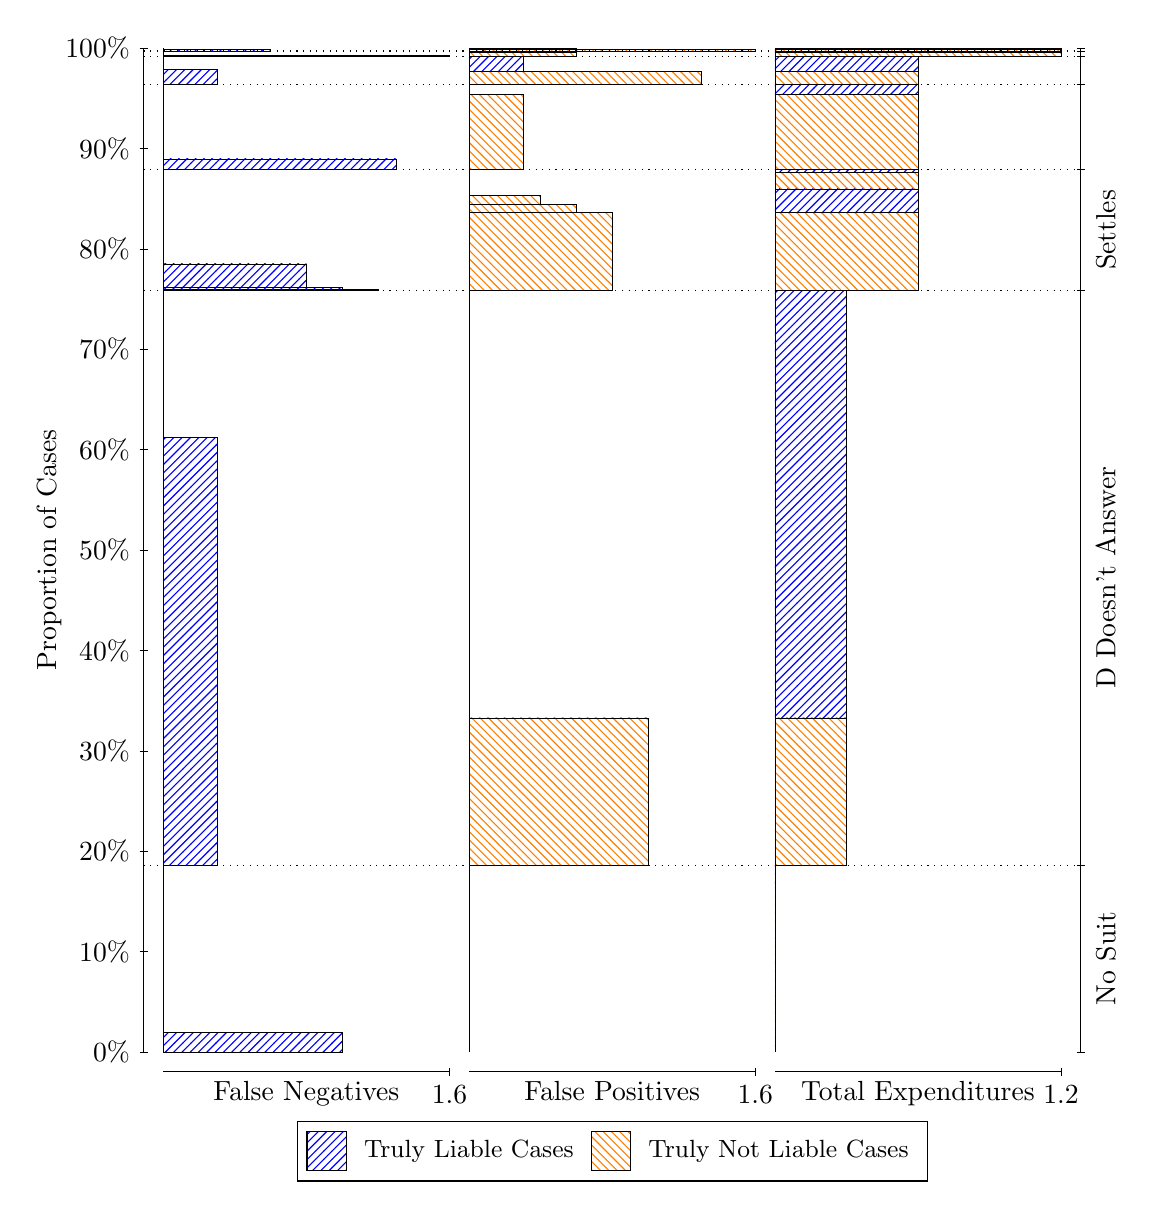
\begin{tikzpicture}
\draw[black, very thin] (1.5,1.75) -- (1.5,14.5);
\node[rotate=90, anchor=center] at (0.3, 8.125) {Proportion of Cases};
\draw[black, very thin] (1.45,1.75) -- (1.55,1.75);
\node[anchor=east] at (1.45, 1.75) {0\%};
\draw[black, very thin] (1.45,3.025) -- (1.55,3.025);
\node[anchor=east] at (1.45, 3.025) {10\%};
\draw[black, very thin] (1.45,4.3) -- (1.55,4.3);
\node[anchor=east] at (1.45, 4.3) {20\%};
\draw[black, very thin] (1.45,5.575) -- (1.55,5.575);
\node[anchor=east] at (1.45, 5.575) {30\%};
\draw[black, very thin] (1.45,6.85) -- (1.55,6.85);
\node[anchor=east] at (1.45, 6.85) {40\%};
\draw[black, very thin] (1.45,8.125) -- (1.55,8.125);
\node[anchor=east] at (1.45, 8.125) {50\%};
\draw[black, very thin] (1.45,9.4) -- (1.55,9.4);
\node[anchor=east] at (1.45, 9.4) {60\%};
\draw[black, very thin] (1.45,10.675) -- (1.55,10.675);
\node[anchor=east] at (1.45, 10.675) {70\%};
\draw[black, very thin] (1.45,11.95) -- (1.55,11.95);
\node[anchor=east] at (1.45, 11.95) {80\%};
\draw[black, very thin] (1.45,13.225) -- (1.55,13.225);
\node[anchor=east] at (1.45, 13.225) {90\%};
\draw[black, very thin] (1.45,14.5) -- (1.55,14.5);
\node[anchor=east] at (1.45, 14.5) {100\%};

\draw[black, very thin] (13.4,1.75) -- (13.4,14.5);
\draw[black, very thin] (13.35,1.75) -- (13.45,1.75);
\node[anchor=west] at (13.35, 1.75) {};
\draw[black, very thin] (13.35,4.1224) -- (13.45,4.1224);
\node[anchor=west] at (13.35, 4.1224) {};
\draw[black, very thin] (13.35,11.424) -- (13.45,11.424);
\node[anchor=west] at (13.35, 11.424) {};
\draw[black, very thin] (13.35,12.959) -- (13.45,12.959);
\node[anchor=west] at (13.35, 12.959) {};
\draw[black, very thin] (13.35,14.041) -- (13.45,14.041);
\node[anchor=west] at (13.35, 14.041) {};
\draw[black, very thin] (13.35,14.389) -- (13.45,14.389);
\node[anchor=west] at (13.35, 14.389) {};
\draw[black, very thin] (13.35,14.462) -- (13.45,14.462);
\node[anchor=west] at (13.35, 14.462) {};
\draw[black, very thin] (13.35,14.5) -- (13.45,14.5);
\node[anchor=west] at (13.35, 14.5) {};

\draw[black, very thin, pattern color=blue, pattern=north east lines] (1.75,1.75) rectangle (4.0208,1.9996);
\draw[black, very thin, pattern color=orange, pattern=north west lines] (1.75,1.9996) rectangle (1.75,4.1224);
\draw[black, very thin, pattern color=blue, pattern=north east lines] (1.75,4.1224) rectangle (2.4312,9.5524);
\draw[black, very thin, pattern color=orange, pattern=north west lines] (1.75,9.5524) rectangle (1.75,11.424);
\draw[black, very thin, pattern color=blue, pattern=north east lines] (1.75,11.424) rectangle (4.475,11.436);
\draw[black, very thin, pattern color=blue, pattern=north east lines] (1.75,11.436) rectangle (4.0208,11.458);
\draw[black, very thin, pattern color=blue, pattern=north east lines] (1.75,11.458) rectangle (3.5667,11.758);
\draw[black, very thin, pattern color=orange, pattern=north west lines] (1.75,11.758) rectangle (1.75,12.959);
\draw[black, very thin, pattern color=blue, pattern=north east lines] (1.75,12.959) rectangle (4.7021,13.092);
\draw[black, very thin, pattern color=orange, pattern=north west lines] (1.75,13.092) rectangle (1.75,14.041);
\draw[black, very thin, pattern color=blue, pattern=north east lines] (1.75,14.041) rectangle (2.4312,14.232);
\draw[black, very thin, pattern color=orange, pattern=north west lines] (1.75,14.232) rectangle (1.75,14.389);
\draw[black, very thin, pattern color=blue, pattern=north east lines] (1.75,14.389) rectangle (5.3833,14.408);
\draw[black, very thin, pattern color=orange, pattern=north west lines] (1.75,14.408) rectangle (1.75,14.462);
\draw[black, very thin, pattern color=blue, pattern=north east lines] (1.75,14.462) rectangle (3.1125,14.482);
\draw[black, very thin, pattern color=orange, pattern=north west lines] (1.75,14.482) rectangle (1.75,14.5);
\draw[black, very thin, pattern color=orange, pattern=north west lines] (5.6333,1.75) rectangle (5.6333,3.8728);
\draw[black, very thin, pattern color=blue, pattern=north east lines] (5.6333,3.8728) rectangle (5.6333,4.1224);
\draw[black, very thin, pattern color=orange, pattern=north west lines] (5.6333,4.1224) rectangle (7.9042,5.9941);
\draw[black, very thin, pattern color=blue, pattern=north east lines] (5.6333,5.9941) rectangle (5.6333,11.424);
\draw[black, very thin, pattern color=orange, pattern=north west lines] (5.6333,11.424) rectangle (7.45,12.41);
\draw[black, very thin, pattern color=orange, pattern=north west lines] (5.6333,12.41) rectangle (6.9958,12.513);
\draw[black, very thin, pattern color=orange, pattern=north west lines] (5.6333,12.513) rectangle (6.5417,12.625);
\draw[black, very thin, pattern color=blue, pattern=north east lines] (5.6333,12.625) rectangle (5.6333,12.959);
\draw[black, very thin, pattern color=orange, pattern=north west lines] (5.6333,12.959) rectangle (6.3146,13.909);
\draw[black, very thin, pattern color=blue, pattern=north east lines] (5.6333,13.909) rectangle (5.6333,14.041);
\draw[black, very thin, pattern color=orange, pattern=north west lines] (5.6333,14.041) rectangle (8.5854,14.199);
\draw[black, very thin, pattern color=blue, pattern=north east lines] (5.6333,14.199) rectangle (6.3146,14.389);
\draw[black, very thin, pattern color=orange, pattern=north west lines] (5.6333,14.389) rectangle (6.9958,14.444);
\draw[black, very thin, pattern color=blue, pattern=north east lines] (5.6333,14.444) rectangle (5.6333,14.462);
\draw[black, very thin, pattern color=orange, pattern=north west lines] (5.6333,14.462) rectangle (9.2667,14.481);
\draw[black, very thin, pattern color=blue, pattern=north east lines] (5.6333,14.481) rectangle (6.9958,14.5);
\draw[black, very thin, pattern color=orange, pattern=north west lines] (9.5167,1.75) rectangle (9.5167,3.8728);
\draw[black, very thin, pattern color=blue, pattern=north east lines] (9.5167,3.8728) rectangle (9.5167,4.1224);
\draw[black, very thin, pattern color=orange, pattern=north west lines] (9.5167,4.1224) rectangle (10.425,5.9941);
\draw[black, very thin, pattern color=blue, pattern=north east lines] (9.5167,5.9941) rectangle (10.425,11.424);
\draw[black, very thin, pattern color=orange, pattern=north west lines] (9.5167,11.424) rectangle (11.333,12.41);
\draw[black, very thin, pattern color=blue, pattern=north east lines] (9.5167,12.41) rectangle (11.333,12.71);
\draw[black, very thin, pattern color=orange, pattern=north west lines] (9.5167,12.71) rectangle (11.333,12.925);
\draw[black, very thin, pattern color=blue, pattern=north east lines] (9.5167,12.925) rectangle (11.333,12.959);
\draw[black, very thin, pattern color=orange, pattern=north west lines] (9.5167,12.959) rectangle (11.333,13.909);
\draw[black, very thin, pattern color=blue, pattern=north east lines] (9.5167,13.909) rectangle (11.333,14.041);
\draw[black, very thin, pattern color=orange, pattern=north west lines] (9.5167,14.041) rectangle (11.333,14.199);
\draw[black, very thin, pattern color=blue, pattern=north east lines] (9.5167,14.199) rectangle (11.333,14.389);
\draw[black, very thin, pattern color=orange, pattern=north west lines] (9.5167,14.389) rectangle (13.15,14.444);
\draw[black, very thin, pattern color=blue, pattern=north east lines] (9.5167,14.444) rectangle (13.15,14.462);
\draw[black, very thin, pattern color=orange, pattern=north west lines] (9.5167,14.462) rectangle (13.15,14.481);
\draw[black, very thin, pattern color=blue, pattern=north east lines] (9.5167,14.481) rectangle (13.15,14.5);
\draw[black, dotted] (1.5,4.1224) -- (13.4,4.1224);
\draw[black, dotted] (1.5,11.424) -- (13.4,11.424);
\draw[black, dotted] (1.5,12.959) -- (13.4,12.959);
\draw[black, dotted] (1.5,14.041) -- (13.4,14.041);
\draw[black, dotted] (1.5,14.389) -- (13.4,14.389);
\draw[black, dotted] (1.5,14.462) -- (13.4,14.462);
\draw[black, very thin] (1.75,1.5) -- (5.3833,1.5);
\node[anchor=north] at (3.5667, 1.5) {False Negatives};
\draw[black, very thin] (5.3833,1.45) -- (5.3833,1.55);
\node[anchor=north] at (5.3833, 1.45) {1.6};

\draw[black, very thin] (5.6333,1.5) -- (9.2667,1.5);
\node[anchor=north] at (7.45, 1.5) {False Positives};
\draw[black, very thin] (9.2667,1.45) -- (9.2667,1.55);
\node[anchor=north] at (9.2667, 1.45) {1.6};

\draw[black, very thin] (9.5167,1.5) -- (13.15,1.5);
\node[anchor=north] at (11.333, 1.5) {Total Expenditures};
\draw[black, very thin] (13.15,1.45) -- (13.15,1.55);
\node[anchor=north] at (13.15, 1.45) {1.2};

\node[black, centered, rotate=90] at (13.72, 2.9362) {No Suit};
\node[black, centered, rotate=90] at (13.72, 7.7733) {D Doesn't Answer};
\node[black, centered, rotate=90] at (13.72, 12.191) {Settles};





\draw (7.449999999999999,1.5) node[draw=none] (baseCoordinate) {};
\begin{scope}[align=center]
        \matrix[scale=0.5, draw=black, below=0.5cm of baseCoordinate, nodes={draw}, column sep=0.1cm]{
            \node[rectangle, draw, minimum width=0.5cm, minimum height=0.5cm, pattern=north east lines, pattern color=blue] {}; &
            \node[draw=none, font=\small] (B) {Truly Liable Cases}; &
            \node[rectangle, draw, minimum width=0.5cm, minimum height=0.5cm, pattern=north west lines, pattern color=orange] {}; &
            \node[draw=none, font=\small] (B) {Truly Not Liable Cases}; \\
            };
\end{scope}

\end{tikzpicture}
\end{document}